\documentclass[twocolumn]{article}

\usepackage{graphicx}
\usepackage[margin=1in]{geometry}
\PassOptionsToPackage{hyphens}{url}\usepackage{hyperref}
\usepackage{url}
\usepackage{cite}

\title{HotSpots: Reducing Contention on Hot Leaves in B-trees}
\date{}
\author{Somya Arora, Mark Mansi, Mohammed Danish Shaikh}

\begin{document}

\maketitle

\begin{abstract}
B-Tree indices are heavily used in modern transactional database systems for
efficient search and range queries. Concurrency in these systems is maximized
by locking at fine granularity. Lock contention among writers can be a severe
performance bottleneck. In particular, when insertions are on a sequential key,
all threads will contend for the rightmost leaf of the B-tree. We propose an
Auxiliary Structure to augment concurrent B-trees and reduce contention. We
evaluate our design against a concurrent B-tree using Optimistic Lock Coupling
(OLC) \cite{art} and an implementation we call byte-reordering that solves contention
but does not support range queries. We find that in the OLC implementation,
lookups scale well with number of threads but insertions do not. We find that
byte-reordering is very effective at reducing contention and is a viable
solution if the use case does not require range scans. Due to implementation
difficulties, we were not able to optimize our Auxiliary Structure’s
performance, so it’s performance lags significantly behind that of the other
implementations; however, we believe more engineering effort is required to
evaluate the full potential of this idea. Finally, we summarize some lessons
learned regarding the design and implementation of concurrent data structures.
\end{abstract}

\section{Introduction}
The B-tree has become a standard access method for database systems owing to
its efficient search, versatility, easy-to-maintain structure, and good
performance on hard drives. Minimal locking strategies for B-trees are also
well known \cite{blink}.

Our paper focuses on the case of a B-tree index on a sequential attribute (that
is, an attribute for which consecutive elements are sequential in the
key-space). If the workload has heavy concurrent record insertions on such a
sequential attribute, then all threads will contend on the same rightmost leaf
node of the B-tree index.  We call such a leaf node with contention, a hot
spot.

For example, suppose that the following B-Tree represents an index on a Sales
table of a database, which is keyed by an auto-incremented order ID. Note that
insertions for orders 19, 20, and 21 will all lock the same page. Additionally,
in order to split the rightmost leaf, we will need to lock the entire path up
to the root of the B-Tree. The contention on rightmost leaf, the hot-spot, is
what we aim to solve in this work.

TODO: image

To mitigate contention on hot spots, we propose a modification to B-trees with
Optimistic Lock Coupling (OLC) \cite{art}: maintaining an auxiliary structure to keep
a track of hot pages. The pages are identified to be hot through maintained
statistics. An insertion to a hot page would update the auxiliary structure
with this information, rather than the B-tree. Searches for a given key first
look in the auxiliary structure. The auxiliary structure uses traditional
locking and concurrent data structures, rather than OLC, to tolerate contention
while attempting to maintain reasonable performance.

A user-defined policy determines which pages are stored in the auxiliary
structure, based on statistics. When a page is evicted from the auxiliary
structure, it is inserted back to the B-tree. This amortizes the cost of
locking the hot area of the B-Tree over many operations.

Our B-tree design can efficiently support all major common index operations,
including insertions, deletions, range scans, and point lookups, though our
prototype implements only insertions and point lookups.

We evaluate our technique’s performance against B-Trees with OLC and against a
solution that reduces contention at the expense of range scans called
byte-reordering. We find that in the OLC implementation, lookups scale well
with number of threads but insertions do not. We find that byte-reordering is
very effective at reducing contention and is a viable solution if the use case
does not require range scans. Due to implementation difficulties, we were not
able to optimize our Auxiliary Structure’s performance, so it’s performance
lags significantly behind that of the other implementations; however, we
believe more engineering effort is required to evaluate the full potential of
this idea. Finally, we summarize some lessons learned regarding the design and
implementation of concurrent data structures.

\section{Background}

Our design is a modification of B-trees with Optimistic Lock Coupling (OLC)
\cite{art}. In this section, we give a brief summary of OLC.

OLC is a locking technique in which writers acquire a traditional lock on nodes
they need to update, while readers optimistically attempt to access data
without acquiring a lock, restarting if there is a conflict with a writer.
Moreover, as in normal Lock Coupling, at any given time, a writer holds at most
two locks, while a reader never waits for locks.

Each node in the B-tree has an associated optimistic lock, which consists of a
version counter and a traditional mutex lock. Each writer must acquire the
mutex on nodes they wish to modify, possibly blocking until another writer
releases the mutex. When a writer releases the mutex, it updates the version
counter associated with the optimistic lock. When a reader wishes to read a
node’s contents, it will first read the version counter (but not acquire the
mutex). When the reader is done, it must check if the version has changed
during its read, indicating a conflict with a writer. If the version has
changed, the reader must restart; otherwise, the reader is done. Care must be
taken to handle deletions properly since a thread might be using a node when it
is deleted. Many concurrent B-tree implementations use epoch-based techniques
to handle deletion safely \cite{bwtree, art}.

Like other optimistic techniques, optimistic lock coupling has higher
performance when conflicts are rare, since this decreases the probability that
a thread must restart. In contrast, traditional locking techniques may have
higher performance when conflicts are frequent, such as when there is a lot of
contention on a hot node \cite{occ}. Our work aims to improve the performance of OLC
under cases where there is contention on a few hot B-tree nodes.

\section{Design}

To reduce contention on pages in the B-tree, we propose a modification to
B-trees with OLC. The key idea is to collect writes to hot pages efficiently in
an auxiliary structure and then amortize the cost of locking the hot area of
B-Tree over many operations when evicting the range from the auxiliary
structure. Since B-Tree indices are secondary data stores, they can be slightly
out of date from the primary store in the case of a crash. We suggest that
during recovery, the lost updates can be rebuilt, though we do not explore
crash recovery further in our work. Our approach attempts to achieve higher
performance by designing the auxiliary structure with contention in mind while
allowing the rest of data to use OLC.

Our design separates policy and mechanism:

\paragraph{Mechanism} Our design augments the B-tree with an auxiliary
structure that aims to allow higher-performance concurrent access to data with
high contention. The auxiliary structure keeps track of ranges of the
key-space. For each range, key-value pairs inserted into the ranges are
diverted from the B-tree to the auxiliary structure, rather than being inserted
into the B-tree. The auxiliary structure uses traditional fine-grain locking to
handle concurrency with high contention.

\paragraph{Policy} The auxiliary structure adds and evicts ranges of keys based
on the policy in use. For our prototype, we use an LRU policy to enforce a
maximum size on the auxiliary data structure.

\subsection{Auxiliary Structure}

The auxiliary structure (AS) is conceptually a concurrent map. It keeps track
of ranges of the key-space as directed by policy. For each range, the AS stores
all key-value pairs inserted into the range. Writes to a single range are
insertions on a concurrent hashmap structure.

Updates to the set of tracked ranges are directed by the policy. Insertions and
deletions of new ranges are serialized using a mutex. We expect these to be
uncommon, so the impact of serialization should be low. When a range is chosen
to be evicted from the AS, it is inserted into the B-tree.

\subsection{Policy}

The policy must be able to handle two possible queries:

\begin{enumerate}
\item ``Is a key in a hot range?'' This is used to determine if an insertion
should be redirected to the AS.
\item ``Mark range [low, high) as touched.'' This is used to update stats used
by the policy to make decisions. This query may also return a range to evict
from the AS.
\end{enumerate}

The policy is completely decoupled from the AS, so different policies can be
plugged in. In principle, it may be possible for the user to supply an
arbitrary policy; however, we do not explore this idea further in our work.

\subsection{B-tree Search and Insertion}

Insertions and searches in the B-tree operate largely as described in prior
work \cite{art, critique}. In this section we describe briefly our
modifications to insertion and search to use the AS and policy.

Search first checks if the key is present in the AS. If the key being searched
for is not present in the AS, a normal B-Tree lookup is performed. The policy
is not informed of access because reads do not contend with each other.

On an insertion, if the policy indicates that the key is in a hot range, the
new pair is inserted into the AS. This may require traversing the B-tree once
to find out the maximum and minimum values that can land on the key’s B-tree
leaf node. This is the range inserted into the AS. Otherwise, if the key is not
in a hot range, it is inserted into the B-tree using the traditional algorithm.
Ranges from the AS are evicted to the B-Tree based on policy as mentioned
above. We use a special bulk-insertion operation to amortize locking over many
keys.

\subsection{Byte-Reordering}

We also evaluate a solution that reorders the bytes of a key in a specific way
to mitigate contention at the expense of range queries. In this solution, we
swap the greatest and least bytes of keys before using them for B-tree
operations. We call this solution byte-reordering. Byte reordering
redistributes consecutive keys to different leaves. This means that threads
inserting sequential values no longer contend on the rightmost leaf.
Unfortunately, it also means that range queries are inefficient.

\section{Implementation}

Our implementation is available at \url{https://github.com/mark-i-m/hot-spots}.
We borrow the B-tree OLC implementation directly from
\url{https://github.com/wangziqi2016/index-microbench} \cite{art}. Our other
implementations are modifications of this implementation.

All implementations are written in C++. Byte-reordering consists of a 73 line
change from the OLC implementation. The hybrid implementation with our
auxiliary structure consists of 757 lines changed. In addition, we use the
concurrent hash map found at \url{https://github.com/efficient/libcuckoo}.

\section{Experimental Evaluation}

\subsection{Methodology}

We evaluate our design by comparing read and sequential write performance to
B-trees with OLC and byte-reordering.

For each implementation, we evaluate throughput and scalability of lookups and
insertions. We run a series of experiments in which we measure the number of
operations per second for a given number of reader threads (threads that only
do lookups) and writer threads (threads that only do insertions). To measure
performance of lookups, we hold the number of writer threads constant and vary
the number of reader threads. Likewise, to measure performance of insertions,
we hold the number of reader threads constant and vary the number of writer
threads. All read operations are point lookups on a random key. All write
operations are sequential, leading to high lock contention.

For our experiments measuring insertion performance we fix the number of reader
threads at 20 and vary the number of writer threads from 1 to 20, and vice
versa for our experiments measuring lookup performance. Each thread performs
100 million operations on the tree. For each experiment, the B-tree under test
is initialized with 1 billion key/value pairs before any measurements are
taken.

Though they are possible to implement, range searches and deletions have not
been implemented or evaluated in this project due to time constraints. We leave
this to future contributions and research.

All experiments were run on CloudLab c220g2 instances with 40 logical cores
(Intel Xeon E5-2660 v3) and 160GB RAM. All B-trees are in-memory. Before each
experiment, we set scaling governors to “performance” on all cores. Each thread
is pinned to its own core. We use `rdtsc` for acquiring timing information.

\subsection{Results}

\paragraph{OLC}

Figure \ref{fig:olclookup} shows the lookup performance of the OLC
implementation. As the figure shows, the reader throughput scales nearly
linearly with the number of threads, achieving a maximum throughput of 17.5
million operations per second with 20 threads.

\begin{figure}[ht]
    \centering 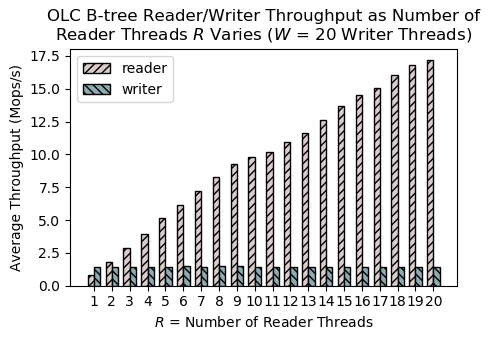
\includegraphics[width=\columnwidth]{figures/olc_w20_r1-20_avg.png}
    \caption{Lookups with OLC \label{fig:olclookup}}
\end{figure}

Figure \ref{fig:olcinsert} shows the insertion performance of the OLC
implementation. As the figure shows, the writer throughput scales linearly up
to 4 threads, reaching a peak throughput of 11 million operations per second.
After that, performance drops to about 2.5 million operations per second. This
experiment demonstrates that insertions under contention do not scale in the
OLC implementation.

\begin{figure}[ht]
    \centering 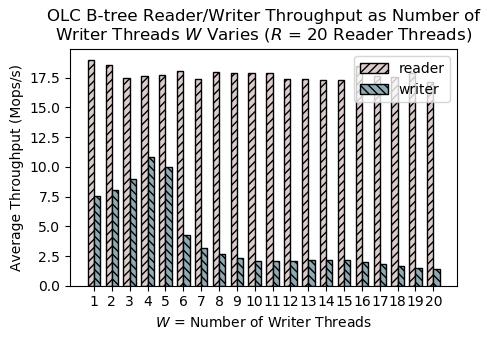
\includegraphics[width=\columnwidth]{figures/olc_r20_w1-20_avg.png}
    \caption{Insertions with OLC \label{fig:olcinsert}}
\end{figure}

\paragraph{Byte-reordering}

Figure \ref{fig:brlookup} shows the lookup performance of the byte-reordering
implementation. As the figure shows, reader throughput matches that of the OLC
implementation.

\begin{figure}[ht]
    \centering 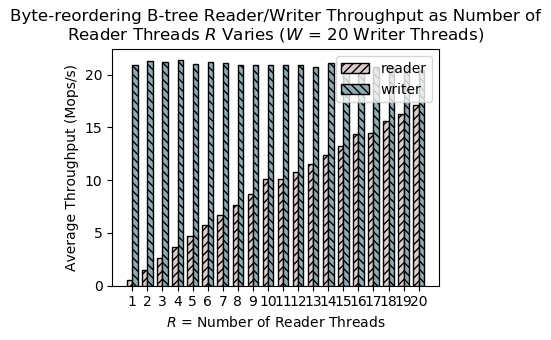
\includegraphics[width=\columnwidth]{figures/br_w20_r1-20_avg.png}
    \caption{Lookups with Byte-reordering \label{fig:brlookup}}
\end{figure}

Figure \ref{fig:brinsert} shows the insertion performance of the
byte-reordering implementation. Unlike the OLC implementation, the
byte-reordering implementation demonstrates linear scalability with number of
threads, reaching a peak throughput of over 20 million operations per second.
This demonstrates that byte-reordering is effective at mitigating hot spots. If
range queries are not needed, byte-reordering is a viable solution.

\begin{figure}[ht]
    \centering 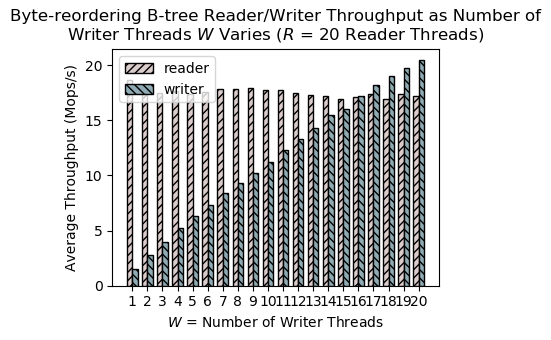
\includegraphics[width=\columnwidth]{figures/br_r20_w1-20_avg.png}
    \caption{Insertions with Byte-reordering \label{fig:brinsert}}
\end{figure}

\paragraph{Hybrid B-tree with Auxiliary Structure}

Figures \ref{fig:hylookup} and \ref{fig:hyinsert} show the lookup and insertion
performance respectively. As the figures show, our design has significantly
poorer performance than either of the other designs. Peak throughput for
lookups was around 2 million operations per second, while peak insertion
throughput was around 0.5 million operations per second. We do observe,
however, that lookups scale with number of threads, suggesting that there may
be promise to our technique.

We believe the poor performance of the hybrid design is largely due to our
implementation. Due to time constraints and the challenges of implementing
concurrent data structures, our implementation had more exclusive locks than we
intended originally. Moreover, we discovered late during implementation that
the concurrent hash map implementation we borrowed does not support any
efficient filtering operation \cite{cuckoo}. Thus, evictions from the caching layer are
extremely inefficient. We believe using a custom-designed caching layer would
significantly improve throughput.

\begin{figure}[ht]
    \centering 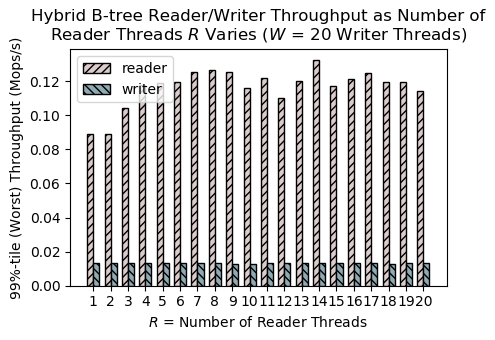
\includegraphics[width=\columnwidth]{figures/hybrid_w20_r1-20_99.png}
    \caption{Lookups with Hybrid \label{fig:hylookup}}
\end{figure}

\begin{figure}[ht]
    \centering 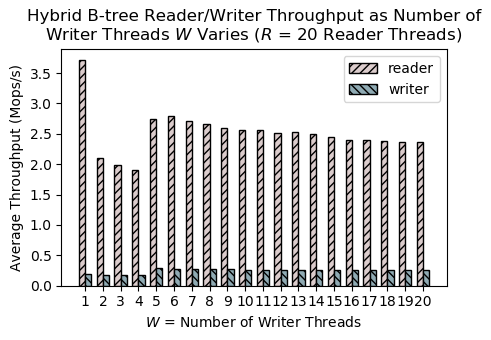
\includegraphics[width=\columnwidth]{figures/hybrid_r20_w1-20_avg.png}
    \caption{Insertions with Hybrid \label{fig:hyinsert}}
\end{figure}


\section{Lessons Learned}

The implementation of the hybrid B-tree with our auxiliary structure was
challenging. This section summarizes lessons we learned in the process.

We began our implementation by designing the policy and caching layers as
independent thread-safe data structures. However, when we tried to “glue” these
data structures together, we found that we had to insert extra locking to make
sure that each data structure stayed synchronized with others.

Also, we found that integrating conventional locking with optimistic methods
and lock-free methods is challenging. For example, a conventional critical
section is nested inside an optimistic critical section, then restarts of the
optimistic critical section may need to release and re-acquire locks. Worse
yet, many operations need to become idempotent to tolerate restarts.

These factors significantly delayed our progress on implementation and
evaluation. In retrospect, we would make the following recommendations:

\begin{enumerate}
\item Design concurrency control first. It is part of the design; it is not an
implementation detail.
\item Design short, incremental critical sections between valid states. This
reduces the size and critical sections and increases concurrency.
\item Replace complex atomic operations by smaller atomic operations, even at a
slight cost in performance.
\item Use formal reasoning, proofs, or other systematic mathematical
techniques. Determine the invariants of your system and enforce them. Then use
them to simplify your thinking about the system. Tests are helpful, but
insufficient.
\end{enumerate}

\section{Related Work}

Bw-Tree is a latch-free B-tree implementation. It makes use of delta nodes to
avoid changing data in place and atomic compare and swap instructions to
transition between consistent B-tree states, eliminating the need for locks
\cite{bwtree}. Since locks aren’t used at all in a Bw-Tree, there is no contention due to
locks in the rightmost leaves. However, follow-up work has suggested that the
extra indirection layer and delta nodes used by Bw-tree outweigh the benefits
of lock-freedom \cite{critique}. In our work, we use a locking-based approach but aim to be
conscientious about lock contention.

B-trees with OLC, as mentioned above, attempt to achieve higher performance by
doing optimistic reads and pessimistic writes \cite{olc, art}. However, we hypothesize
that this approach will have poor performance for workloads with sequential
writes due to reader/writer conflicts. We attempt to modify the B-Tree with OLC
to make it behave efficiently in face of the hotspot problem.

\section{Conclusion}

In this paper, we explore two different techniques for mitigating lock
contention on the rightmost leaf of a B-tree under sequential insertions. We
demonstrate experimentally that such contention is indeed a concern for a
B-tree implementation using OLC. We then demonstrate that byte-reordering is an
effective way of mitigating the concern if one is willing to give up efficient
range scans. We also propose a design for reducing contention using a caching
layer that handles contention well. Our implementation was not
highly-performant, though we did identify some implementation choices that may
be limiting performance. We believe more engineering effort is required to
fully evaluate the approach. Finally, we summarize some lessons we learned
regarding the design and implementation of concurrent data structures.

\section*{Acknowledgements}

We extend our sincere gratitude to Alan Halverson, for providing us an
opportunity to work under him on this project and for his much valuable
suggestions, support and continuous encouragement throughout the duration of
the project. We would also like to thank Ziqi Wang, PhD student at the Computer
Science Department, Carnegie Mellon University, for providing us with the
implementation of B-Tree with Optimistic Lock Control used in prior work \cite{olc, critique}.

\bibliographystyle{plain}
\bibliography{references}

\end{document}
